%%%%%%%%%%%%%%%%%%%%%%%%%%%%%%%%%%%%%%%%%
% Beamer Presentation
% LaTeX Template
% Version 1.0 (10/11/12)
%
% This template has been downloaded from:
% http://www.LaTeXTemplates.com
%
% License:
% CC BY-NC-SA 3.0 (http://creativecommons.org/licenses/by-nc-sa/3.0/)
%
%%%%%%%%%%%%%%%%%%%%%%%%%%%%%%%%%%%%%%%%%

%----------------------------------------------------------------------------------------
%	PACKAGES AND THEMES
%----------------------------------------------------------------------------------------

\documentclass[usenames,dvipsnames]{beamer}

\usepackage{lstautogobble}
\usepackage{ulem}
\usepackage{xcolor}
\definecolor{eclipseBlue}{RGB}{42,0,255}
\definecolor{eclipseGreen}{RGB}{63,127,95}

\mode<presentation> {

% The Beamer class comes with a number of default slide themes
% which change the colors and layouts of slides. Below this is a list
% of all the themes, uncomment each in turn to see what they look like.

%\usetheme{default}
%\usetheme{AnnArbor}
%\usetheme{Antibes}
%\usetheme{Bergen}
%\usetheme{Berkeley}
%\usetheme{Berlin}
%\usetheme{Boadilla}
\usetheme{CambridgeUS}
%\usetheme{Copenhagen}
%\usetheme{Darmstadt}
%\usetheme{Dresden}
%\usetheme{Frankfurt}
%\usetheme{Goettingen}
%\usetheme{Hannover}
%\usetheme{Ilmenau}
%\usetheme{JuanLesPins}
%\usetheme{Luebeck}
%\usetheme{Madrid}
%\usetheme{Malmoe}
%\usetheme{Marburg}
%\usetheme{Montpellier}
%\usetheme{PaloAlto}
%\usetheme{Pittsburgh}
%\usetheme{Rochester}
%\usetheme{Singapore}
%\usetheme{Szeged}
%\usetheme{Warsaw}

% As well as themes, the Beamer class has a number of color themes
% for any slide theme. Uncomment each of these in turn to see how it
% changes the colors of your current slide theme.

%\usecolortheme{albatross}
%\usecolortheme{beaver}
%\usecolortheme{beetle}
%\usecolortheme{crane}
%\usecolortheme{dolphin}
%\usecolortheme{dove}
%\usecolortheme{fly}
%\usecolortheme{lily}
\usecolortheme{orchid}
%\usecolortheme{rose}
%\usecolortheme{seagull}
%\usecolortheme{seahorse}
%\usecolortheme{whale}
%\usecolortheme{wolverine}

%\setbeamertemplate{footline} % To remove the footer line in all slides uncomment this line
%\setbeamertemplate{footline}[page number] % To replace the footer line in all slides with a simple slide count uncomment this line

\setbeamertemplate{navigation symbols}{} % To remove the navigation symbols from the bottom of all slides uncomment this line
}

\usepackage{graphicx} % Allows including images
\usepackage{booktabs} % Allows the use of \toprule, \midrule and \bottomrule in tables
\usepackage{stmaryrd}
\usepackage{amsmath}
\usepackage{environ}
\usepackage{mathtools}
\usepackage[absolute,overlay]{textpos}

\newcommand{\Exp}{\texttt{Exp}}
\newcommand{\compile}{\texttt{compile}}
\newcommand{\syn}{\textsc{Syntax}}
\newcommand{\denot}[2][]{\llbracket #2 \rrbracket_{#1}}

\NewEnviron{totop}{
  \begin{textblock*}{\paperwidth}(1.5em,0.2\textheight)
    \raggedright \BODY \hspace{.5em}
  \end{textblock*}}

\lstnewenvironment{code}[1][]
{\lstset{
  frame=none,
  xleftmargin=2pt,
  stepnumber=1,
  numbers=none,
  belowcaptionskip=\bigskipamount,
  captionpos=b,
  escapeinside={*'}{'*},
  language=Haskell,
  tabsize=2,
  emphstyle={\bf},
  commentstyle=\it,
  stringstyle=\mdseries\rmfamily,
  showspaces=false,
  keywordstyle=\bfseries\rmfamily,
  columns=flexible,
  basicstyle=\small\ttfamily,
  showstringspaces=false,
  morecomment=[l]\%,
  escapeinside={`}{`},
}}{}

\makeatletter
\def\blfootnote{\xdef\@thefnmark{}\@footnotetext}
\makeatother

\newcommand{\N}{\mathbb{N}}

%----------------------------------------------------------------------------------------
%	TITLE PAGE
%----------------------------------------------------------------------------------------

\title[]{Calculating Correct Compilers} % The short title appears at the bottom of every slide, the full title is only on the title page

\author{Cameron Wong} % Your name
\institute[CS-252R]{Bahr/Hutton 2015, Pickard/Hutton 2021}
\date{2022-11-03} % Date, can be changed to a custom date

\begin{document}

\begin{frame}
\titlepage % Print the title page as the first slide
\end{frame}

%\begin{frame}
%\frametitle{Overview} % Table of contents slide, comment this block out to remove it
%\tableofcontents % Throughout your presentation, if you choose to use \section{} and \subsection{} commands, these will automatically be printed on this slide as an overview of your presentation
%\end{frame}

%------------------------------------------------------------------------------
%	PRESENTATION SLIDES
%------------------------------------------------------------------------------

%------------------------------------------------

\begin{frame}
  \frametitle{}

  \begin{center}
    \Huge Calculating Correct \textcolor{red}{Compilers}
  \end{center}
\end{frame}

%------------------------------------------------

\begin{frame}
  \frametitle{Compilers?}

  \begin{itemize}
    \item Let $S$ and $T$ be programming languages
    \item We define a compiler from $S$ to $T$ to be a function
      \begin{equation}
        \compile : \syn_{S} \rightarrow \syn_{T}
      \end{equation}
      where
      \begin{itemize}
        \item $S$ is the \emph{source} (or \emph{surface}) language
        \item $T$ is the \emph{target} language
      \end{itemize}
  \end{itemize}
\end{frame}

%------------------------------------------------

\begin{frame}
  \frametitle{Compilers?}

  \begin{itemize}
    \item Usually, we also want an actual implementation of the \compile{}
      function

    \item This implementation language is called the \emph{host} language
  \end{itemize}
\end{frame}

%------------------------------------------------

\begin{frame}
  \frametitle{Compilers?}

  \begin{itemize}
    \item Ignore practical details like parsing, linking, etc

    \item For simplicity, assume that the input is well-behaved (no type
      errors, etc)

    \item This means that the \compile{} function is a \emph{total} function
      from syntax to syntax
  \end{itemize}
\end{frame}

%------------------------------------------------

\begin{frame}
  \frametitle{}

  \begin{center}
    \Huge Calculating \textcolor{red}{Correct} Compilers
  \end{center}
\end{frame}

%------------------------------------------------

\begin{frame}
  \frametitle{Correct?}

  \begin{itemize}
    \item Languages are defined by their \emph{syntax} and \emph{semantics}
    \item If \compile{} acts on syntax, its \textit{correctness} should talk
      about semantics
  \end{itemize}
\end{frame}

%------------------------------------------------

\begin{frame}
  \frametitle{Correct?}

  \begin{itemize}
    \item What can we say about semantics?
  \end{itemize}
\end{frame}

%------------------------------------------------

\begin{frame}
  \frametitle{Correct?}

  \begin{itemize}
    \item $e$ and $\compile\ e$ should "mean the same thing"
    \item Let's restrict even further to \emph{dynamic} (runtime) correctness
      \begin{itemize}
        \item $e$ and $\compile\ e$ should "\emph{do} the same thing"
      \end{itemize}
  \end{itemize}
\end{frame}

%------------------------------------------------

\begin{frame}
  \frametitle{Correct?}

  \begin{itemize}
    \item This is actually very difficult to state formally!
  \end{itemize}
\end{frame}

%------------------------------------------------

\begin{frame}
  \frametitle{Correct?}

  \begin{itemize}
    \item What \emph{parts} of behavior need to be preserved?
      \begin{itemize}
        \item Performance?
        \item Memory?
      \end{itemize}

    \item $S$ and $T$ may not even use the same execution model! Think
      \begin{itemize}
        \item $S =$ lambda calculus
        \item $T =$ turing machines
      \end{itemize}
  \end{itemize}
\end{frame}

%------------------------------------------------

\begin{frame}
  \frametitle{Correct?}

  \begin{itemize}
    \item Even just looking at "return values" takes some machinery

    \item Suppose
      \begin{itemize}
        \item $e \rightsquigarrow^* v$ and
        \item $\compile\ e \rightsquigarrow^* \overline{v}$
      \end{itemize}

    \item $v$ is in $S$, but $\overline{v}$ is in $T$!

    \item For example, if $S$ is Java and $T$ is assembly, $v$ could be some
      a complex object!
  \end{itemize}
\end{frame}

%------------------------------------------------

\begin{frame}
  \frametitle{Correct?}

  \begin{itemize}
    \item Idea: define a relation $R$ on $\text{values}(S) \times
      \text{values}(T)$

    \item Can then define correctness as
      \begin{itemize}
        \item If $e \rightsquigarrow^* v$ and $\compile\ e \rightsquigarrow^*
          \overline{v}$, then $R(v, \overline{v})$
      \end{itemize}

    \item Could generalize and define the relation over $\syn_S \times \syn_T$,
      but this is typically much harder
  \end{itemize}
\end{frame}

%------------------------------------------------

\begin{frame}
  \frametitle{Correct?}

  \begin{itemize}
    \item Another way: define some common \emph{semantic domain} $D$, with
      \emph{denotation functions}
      \begin{itemize}
        \item $\denot[S]{\cdot} : \text{programs}(S) \rightarrow D$
        \item $\denot[T]{\cdot} : \text{programs}(T) \rightarrow D$
      \end{itemize}

    \item Then correctness is stated as
      \begin{equation}
        \denot[S]{e} = \denot[T]{\compile\ e}
      \end{equation}
  \end{itemize}

  \blfootnote{This is also known as a logical relation}
\end{frame}

%------------------------------------------------

\begin{frame}
  \frametitle{Correct?}

  \begin{itemize}
    \item $D$ and $\denot{\cdot}$ exist outside of the languages $S$ and $T$,
      so they can be arbitrarily complicated

    \item Ex
      \begin{itemize}
        \item Let $D = \mathbb{N} \cup \{ \bot \}$ such that $\denot{e} =
          \bot$ if $e$ infinite-loops when executed
      \end{itemize}
  \end{itemize}
\end{frame}

%------------------------------------------------

\begin{frame}
  \frametitle{Correct?}

  \begin{itemize}
    \item For us: Our approach will look like the denotation method, embedded
      into the host language
      \begin{itemize}
        \item That is, $\denot[S]{\cdot}$ and $\denot[T]{\cdot}$ will be
          host language functions, rather than purely metatheoretical
      \end{itemize}
  \end{itemize}
\end{frame}

%------------------------------------------------

\begin{frame}
  \frametitle{}

  \begin{center}
    \Huge \textcolor{red}{Calculating} Correct Compilers
  \end{center}
\end{frame}

%------------------------------------------------

\begin{frame}[fragile]
  \frametitle{Setup}

  \begin{itemize}
    \item Define the syntax of our source language as follows:

      \begin{code}
        data Expr where
          Val : `$\mathbb{N}$` `$\rightarrow$` Expr
          Add : Expr `$\rightarrow$` Expr `$\rightarrow$` Expr
      \end{code}

      (where $\N$ is the type of natural numbers \emph{in our host language})
  \end{itemize}
\end{frame}

%------------------------------------------------

\begin{frame}[fragile]
  \frametitle{Setup}

  \begin{itemize}
    \item Define the semantics of our source via an interpreter:

      \begin{code}
        eval : Expr `$\rightarrow$` `$\N$`
        eval (Val x) = x
        eval (Add x y) = eval x + eval y
      \end{code}
  \end{itemize}
\end{frame}

%------------------------------------------------

\begin{frame}
  \frametitle{Setup}

  \begin{itemize}
    \item Notice that \texttt{eval} transforms a \emph{source language} term
      into a \emph{host language} value.
    \item This is exactly what we want for our denotation!
  \end{itemize}
\end{frame}

%------------------------------------------------

\begin{frame}
  \frametitle{Target language}

  \begin{itemize}
    \item What about the target language?
  \end{itemize}
\end{frame}

%------------------------------------------------
\newcommand{\Expr}{\texttt{Expr}}

\begin{frame}[fragile]
  \frametitle{Target language?}

  \begin{itemize}
    \item We'll compile \Expr{} to a yet-undefined stack-based language

      \begin{code}
        data Code where
          -- To be determined
      \end{code}
  \end{itemize}
\end{frame}

%------------------------------------------------

\begin{frame}[fragile]
  \frametitle{Target language}

  \begin{itemize}
    \item Since \texttt{eval} outputs a natural number, our stack should
      contain nats:

      \begin{code}
        type Stack = [`$\N$`]
      \end{code}

    \item We'll also define an interpreter on these stacks:

      \begin{code}
        exec : Code `$\rightarrow$` Stack `$\rightarrow$` Stack
      \end{code}
  \end{itemize}
\end{frame}

%------------------------------------------------

\begin{frame}[fragile]
  \frametitle{The Plan}

  \begin{itemize}
    \item Goal: Derive the definitions of \texttt{Code} and \texttt{exec}
      at the same time, using our (TBD) correctness theorem as a guide
    \item As mentioned, we'll use denotations to state the correctness
      principle
  \end{itemize}
\end{frame}

%------------------------------------------------

\begin{frame}[fragile]
  \frametitle{Correctness}

  \begin{itemize}
    \item What to choose for our semantic domain $D$?
  \end{itemize}
\end{frame}

%------------------------------------------------

\begin{frame}[fragile]
  \frametitle{Correctness}

  \begin{itemize}
    \item Since \texttt{eval} returns $\N$, we could choose $D = \N$

    \item Our denotations would be
      \begin{align*}
        \denot[\Expr]{e} &= \texttt{eval}\ e \\
        \denot[\texttt{Code}]{\overline{e}} &=
          \texttt{head}\ (\texttt{exec}\ \overline{e}\ \texttt{[]})
      \end{align*}

    \item This suggests the following correctness theorem:
      \begin{equation}
        \forall e\ .\ \texttt{exec (compile}\ e\texttt{) []} =
        \texttt{eval}\ e :: \texttt{[]}
      \end{equation}

    \item "executing this code from an empty stack gives the right answer"
  \end{itemize}
\end{frame}

%------------------------------------------------

\begin{frame}[fragile]
  \frametitle{Correctness}

  \begin{itemize}
    \item It turns out that this doesn't work!
      \footnote{To see why, try to directly prove this theorem for the final
      \compile{} function we produce at the end}

    \item Instead, we need something stronger:
      \begin{equation}\label{correctness}
        \forall e, s\ .\ \texttt{exec (compile}\ e\texttt{)}\ s =
        \texttt{eval}\ e :: s
      \end{equation}
  \end{itemize}
\end{frame}

%------------------------------------------------

\begin{frame}[fragile]
  \frametitle{Denotations?}

  \begin{itemize}
    \item Aside: What is the denotation function here?
  \end{itemize}
\end{frame}

%------------------------------------------------

\begin{frame}[fragile]
  \frametitle{Denotations?}

  \begin{itemize}
    \item Choose $D = \texttt{Stack} \rightarrow \texttt{Stack}$:

      \begin{align*}
        \denot[\Expr]{e} &= \lambda s . \texttt{eval}\ e :: s \\
        \denot[\texttt{Code}]{\overline{e}} &= \lambda s . \texttt{exec}\ e\ s
      \end{align*}

    \item Define equality as extensional equality, e.g. $f_1 = f_2$ when
      $f_1(x) = f_2(x)$.
  \end{itemize}
\end{frame}

%------------------------------------------------

\begin{frame}[fragile]
  \frametitle{The Plan, restated}

  \begin{itemize}
    \item At last, all the pieces are in place.

    \item The plan:
      \begin{itemize}
        \item Induct on the structure of \Expr{}.

        \item Use equation \ref{correctness} to define \texttt{exec} and
          \texttt{compile}.
      \end{itemize}

    \item Because we used equation \ref{correctness} in this derivation,
      we get the correctness of \texttt{compile} for free!
  \end{itemize}
\end{frame}

%------------------------------------------------

\begin{frame}[fragile]
  \frametitle{Some induction}
  \begin{totop}
    Case: $e = \texttt{Val}\ x$
  \end{totop}

  \begin{itemize}
    \item Want to find \texttt{exec}, $c$ solving

      \begin{equation}
        \texttt{exec}\ c\ s = x :: s
      \end{equation}
  \end{itemize}
\end{frame}

%------------------------------------------------

\begin{frame}[fragile]
  \frametitle{Some induction}
  \begin{totop}
    Case: $e = \texttt{Val}\ x$
  \end{totop}

  \begin{itemize}
    \item Currently, \texttt{Code} has \emph{no} syntax!

    \item So, make a new constructor \texttt{PUSH} for this case.
      \begin{itemize}
        \item $x$ is used on the RHS but doesn't appear on the LHS, so
          \texttt{PUSH} must take $x$ as an argument

        \item Then, define

          \begin{code}
            compile (Var `$x$`) = PUSH `$x$`
            exec (PUSH `$x$`) `$s$` = `$x$` :: `$s$`
          \end{code}
      \end{itemize}
  \end{itemize}
\end{frame}

%------------------------------------------------

\begin{frame}[fragile]
  \frametitle{More induction}
  \begin{totop}
    Case: $e = \texttt{Add}\ e_1\ e_2$
  \end{totop}

  \begin{itemize}
    \item Need to solve

      \begin{equation}
        \texttt{exec}\ c\ s = (\texttt{eval}\ e_1 + \texttt{eval}\ e_2) :: s
      \end{equation}

    \item As before, we define new syntax form \texttt{ADD}
  \end{itemize}
\end{frame}

%------------------------------------------------

\begin{frame}[fragile]
  \frametitle{More induction}
  \begin{totop}
    Case: $e = \texttt{Add}\ e_1\ e_2$
  \end{totop}

  \begin{itemize}
    \item Idea: Have \texttt{Add} take two arguments, as before

      \begin{code}
        compile (Add `$e_1$` `$e_2$`) = ADD (eval `$e_1$`) (eval `$e_2$`)
        exec (ADD `$x$` `$y$`) `$s$` = `$x+y$` :: `$s$`
      \end{code}

    \item Problem: \texttt{compile} uses \texttt{eval}.\footnote{
        We don't actually want to rule out \texttt{eval} entirely; some
        compilers actually will call \texttt{eval} on fragments of the source,
        usually for optimization. We just want to rule out degenerate compilers
        like this one, which cheat by effectively only translating the return
        value.
      }.
  \end{itemize}
\end{frame}

%------------------------------------------------

\begin{frame}[fragile]
  \frametitle{More induction}
  \begin{totop}
    Case: $e = \texttt{Add}\ e_1\ e_2$
  \end{totop}

  \begin{itemize}
    \item Instead, pass arguments to \texttt{ADD} on the stack $s$:

      \begin{code}
        exec ADD `$(x::y::s)$` = `$x+y$` :: `$s$`
      \end{code}
  \end{itemize}
\end{frame}

%------------------------------------------------

\begin{frame}[fragile]
  \frametitle{More induction}
  \begin{totop}
    Case: $e = \texttt{Add}\ e_1\ e_2$
  \end{totop}

  \begin{itemize}
    \item Now, use the inductive hypotheses to define $c$:
      \begin{align*}
          &\texttt{eval }e_1+\texttt{eval }e_2 :: s \\
        = &\ \ \langle \text{definition of }\texttt{exec} \rangle \\
          &\texttt{exec ADD}\ (\texttt{eval }e_1 :: \texttt{eval }e_2 :: s) \\
        = &\ \ \langle \text{inductive hypothesis, $e_1$} \rangle \\
          &\texttt{exec ADD}\ (
            \texttt{exec}\ (\texttt{compile}\ e_1)\ (\texttt{eval }e_2 :: s))
            \\
        = &\ \ \langle \text{inductive hypothesis, $e_2$} \rangle \\
          &\texttt{exec ADD}\ (
            \texttt{exec}\ (\texttt{compile}\ e_1)\ (
              \texttt{exec}\ (\texttt{compile}\ e_2)\ s))
      \end{align*}
  \end{itemize}
\end{frame}

%------------------------------------------------

\begin{frame}[fragile]
  \frametitle{More induction}
  \begin{totop}
    Case: $e = \texttt{Add}\ e_1\ e_2$
  \end{totop}

  \begin{itemize}
    \item We're actually stuck again, so we need to define more syntax

      \begin{code}
        exec (`$c_1$` +++ `$c_2$`) `$s$` = exec `$c_2$` (exec `$c_1$` `$s$`)
      \end{code}

    \item Can finalize with

      \begin{code}
        compile (Add `$e_1$` `$e_2$`) = compile `$e_1$` +++ `$e_2$` +++ ADD
      \end{code}
  \end{itemize}
\end{frame}

%------------------------------------------------

\begin{frame}[fragile]
  \frametitle{Recap}

  \begin{code}
    data Code where
      PUSH : `$\N$` `$\rightarrow$` Code
      ADD : Code
      _+++_ : Code `$\rightarrow$` Code `$\rightarrow$` Code

    compile : Expr `$\rightarrow$` Code
    compile (Var `$x$`) = PUSH x
    compile (Add `$e_1$` `$e_2$`) = compile `$e_1$` +++ `$e_2$` +++ ADD

    exec (PUSH `$x$`) `$s$` = `$x :: s$`
    exec ADD `$(x :: y :: s)$` = `$x + y :: s$`
    exec (`$c_1$` +++ `$c_2$`) `$s$` = exec `$c_2$` (exec `$c_1$` `$s$`)
  \end{code}
\end{frame}

%------------------------------------------------

\begin{frame}[fragile]
  \frametitle{Extensions: Dependent Types}

  \begin{itemize}
    \item Can be used formalize our idea of "well-formed" inputs
    \item Can also be used to make \texttt{exec} more safe (can rule out
      $\texttt{exec ADD []}$)
  \end{itemize}
\end{frame}

%------------------------------------------------

\begin{frame}[fragile]
  \frametitle{Extensions: Exceptions}

  \begin{itemize}
    \item Need to use \emph{code continuations}
      \begin{code}
        compile' : Expr `$\rightarrow$` Code `$\rightarrow$` Code
      \end{code}

    \item Actually, this complicates our denotations:
      \begin{itemize}
        \item The \texttt{compile'} function takes both \Expr{} (source)
          \textit{and} \texttt{Code} (target) arguments

        \item It's not immediately obvious how to define $\denot[\Expr]{\cdot}$
          in this model
      \end{itemize}
  \end{itemize}
\end{frame}

%------------------------------------------------

\begin{frame}[fragile]
  \frametitle{How to represent exceptions?}

  \begin{itemize}
    \item Define a "chained" compiler from \Expr{} to \texttt{Code}:
      \begin{equation*}
        \Expr
          \xrightarrow{\lambda e . (e , \texttt{HALT})}
        \Expr \times \texttt{Code}
          \xrightarrow{\texttt{compile'}}
        \texttt{Code}
      \end{equation*}
      \begin{code}
                  compile `$e$` = compile' `$e$` HALT
      \end{code}

    \item Now we can \emph{switch} denotations halfway!

    \item Correctness of $\lambda e . (e , \texttt{HALT})$ is obvious

    \item Correctness of $\texttt{compile'}$ can be defined straightforwardly:
      \begin{align*}
        D &= \texttt{Stack} \\
        \denot[\Expr \times \texttt{Code}]{(e,c)} &=
          \texttt{exec }c\texttt{ (eval $e :: s$)} \\
        \denot[\texttt{Code}]{(\overline{e},c)} &=
          \texttt{exec (comp $\overline{e}$ $c$) $s$}
      \end{align*}
  \end{itemize}
\end{frame}

%------------------------------------------------

\begin{frame}[fragile]
  \frametitle{Why?}

  \begin{itemize}
    \item Why would we \emph{want} to do this?

    \item What use is a compiler with an unknown target language?
  \end{itemize}
\end{frame}

%------------------------------------------------

\begin{frame}[fragile]
  \frametitle{Some compiler architecture}

  \begin{itemize}
    \item Compilers for real languages don't usually go directly from source to
      target

    \item Instead, they compile through a series of \emph{intermediate
      representations}
  \end{itemize}
\end{frame}

%------------------------------------------------

\begin{frame}[fragile]
  \frametitle{Some compiler architecture}

  \begin{center}
  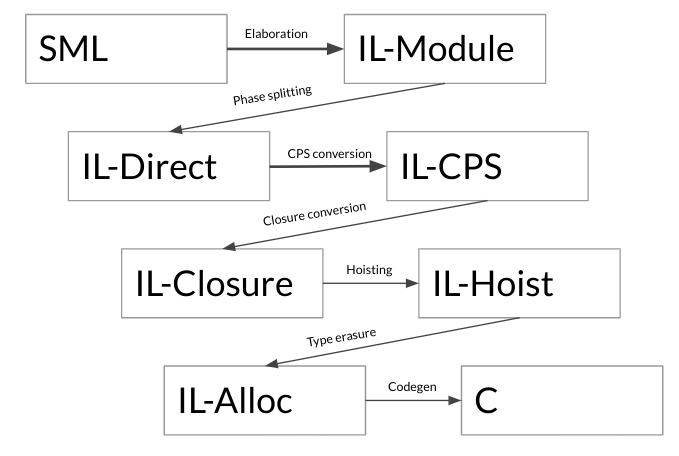
\includegraphics[scale=0.5]{sml-sequence}
  \end{center}
  \blfootnote{Crary 2020, CMU 15-417 Higher-Order Typed Compilation}
\end{frame}

%------------------------------------------------

\begin{frame}[fragile]
  \frametitle{Why?}

  \begin{itemize}
    \item Each of those "IL-" phases are full-fledged programming languages.

    \item If each step is individually correct, then it should\footnote{
        It \textit{is} possible to have compiler phases that are individually
        correct but incorrect when composed (or when composed in a bad order),
        but this tends to arise from incomplete language specifications
      } be correct to pipeline them together!
  \end{itemize}
\end{frame}

%------------------------------------------------

\begin{frame}[fragile]
  \frametitle{More compiler architecture (Glasgow Haskell Compiler)}

  \begin{center}
  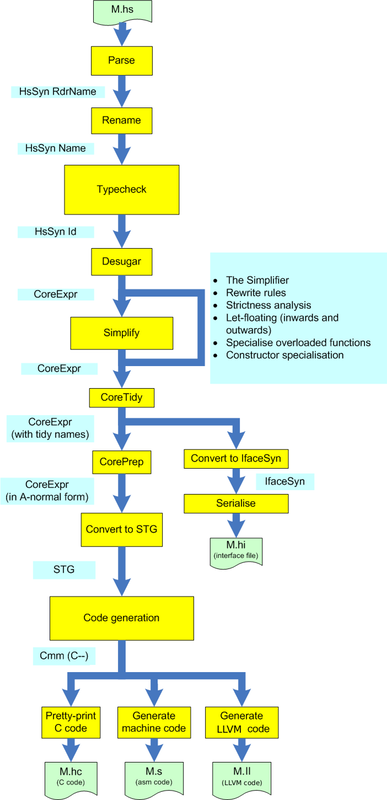
\includegraphics[scale=0.2]{hscpipe2}
  \end{center}
  \blfootnote{Marlow/Peyton-Jones, The Architecture of Open Source
  Applications}
\end{frame}

%------------------------------------------------

\begin{frame}[fragile]
  \frametitle{Why?}

  \begin{itemize}
    \item How were those intermediate forms designed?

    \item The developers constructed them ad-hoc to have certain properties,
      then \emph{separately} reasoned (formally or informally) that the
      translation is correct
  \end{itemize}
\end{frame}

%------------------------------------------------

\begin{frame}[fragile]
  \frametitle{Why?}

  \begin{itemize}
    \item What if we could build the intermediate forms and its translation in a
      correct-by-construction way?
  \end{itemize}
\end{frame}

%------------------------------------------------

\begin{frame}[fragile]
  \frametitle{Question break}
\end{frame}

%------------------------------------------------

\begin{frame}[fragile]
  \frametitle{Final Project Concepts}

  \begin{itemize}
    \item What if we could do all of that, but applied to something else?
  \end{itemize}
\end{frame}

%------------------------------------------------

\begin{frame}[fragile]
  \frametitle{Final Project Concepts}

  \begin{itemize}
    \item What if we could do all of that, but applied to
      \sout{something else} semantics themselves?
  \end{itemize}
\end{frame}

%------------------------------------------------

\begin{frame}[fragile]
  \frametitle{Final Project Concepts}

  \begin{itemize}
    \item Suppose we have the typing rules for some programming language,
      defined by a function
      \begin{code}
        typeof : Expr `$\rightarrow$` Maybe Type
      \end{code}

    \item The most basic notions of type safety are the twin theorems of
      \emph{progress} and \emph{preservation}:
      \begin{itemize}
        \item Progress: Well-typed programs don't get stuck
        \item Preservation: Well-typed programs remain well-typed
      \end{itemize}
  \end{itemize}
\end{frame}

%------------------------------------------------

\begin{frame}[fragile]
  \frametitle{Final Project Concepts}

  \begin{itemize}
    \item What can equational reasoning tell us about these theorems?

    \item Progress can be witnessed by a function
      \begin{code}
        data Progress : Set where
          STEP : Expr `$\rightarrow$`  Progress
          DONE : Progress

        progress : (e : Expr) `$\rightarrow$` `$\exists \tau .$`(typeof e `$\equiv \tau$`) `$\rightarrow$` Progress
      \end{code}

    \item If we assume all expressions are well-typed and \texttt{DONE} for
      now, we get
      \begin{code}
        step : Expr `$\rightarrow$` Expr
      \end{code}
  \end{itemize}
\end{frame}

%------------------------------------------------

\begin{frame}[fragile]
  \frametitle{Final Project Concepts}

  \begin{itemize}
    \item This means we can define preservation as the equation
      \begin{code}
        typeof (step `$e$`) = typeof `$e$`
      \end{code}
      (ignoring ill-typed expressions and values for brevity)
  \end{itemize}
\end{frame}

%------------------------------------------------

\begin{frame}[fragile]
  \frametitle{Final Project Concepts}

  \begin{itemize}
    \item Can we use this equation, and the definition of \texttt{typeof}, to
      construct an appropriate definition of \texttt{step}?

    \item \mbox{}\onslide<2-> (Yes, it works, and it's so trivial that it got
      rejected from a workshop earlier this year)
  \end{itemize}
\end{frame}

%------------------------------------------------

\begin{frame}[fragile]
  \frametitle{Making it cooler}

  \begin{itemize}
    \item Could we derive the \texttt{typeof} function itself? (from
      \texttt{step}? From the inference rules?)
    \item Does this generalize to more interesting systems?
    \item Can we generate the interpreter mechanically, instead of performing
      the calculation by hand?
  \end{itemize}
\end{frame}

%------------------------------------------------

\begin{frame}[fragile]
  \frametitle{Idea: Gradual typing}

  \begin{itemize}
    \item In a gradually-typed system, we have the "gradual guarantee":
      \begin{center}
        "Replacing a type annotation with \texttt{dyn} won't change the result"
      \end{center}

    \item Can we phrase this as an equation? Something like
      \begin{equation}
        \texttt{eval (gradualize $e$)} = \texttt{eval }e
      \end{equation}

    \item Is this sufficient to derive \texttt{eval}?
      \begin{itemize}
        \item Probably not, but maybe with some additional constraints
      \end{itemize}
  \end{itemize}
\end{frame}

\end{document}
